\documentclass{beamer}
\usepackage{amsthm}
\usepackage{times}
\usepackage{graphicx}
\usefonttheme{professionalfonts}
\usetheme{metropolis}
%\usepackage{subcaption}
\usepackage{wrapfig}
\usepackage{media9}
\usepackage{multimedia}
\usepackage{tikz}
%\usecolortheme{sidebartab}
\title{Data analysis and modeling of  calcium activity in   mice somatostatin interneurons}
%\subtitle{L'equazione di Fisher}
\author[F. Bernardi]{\textbf{Fabrizio Bernardi} (944476) \\
	Advisor: Prof. Riccardo Sacco \\
	Coadvisor: Dott. Francesco Papaleo \\
	Coadvisor: Dott. Greta Chiaravalli} \medskip
%\titlegraphic{
\includegraphics[scale=.1]{Logo_Politecnico_Milano.jpg}}
%\titlegraphic{
\includegraphics[scale=.3]{Logo_IIT.png}}
%\usecolortheme{beaver}

\date[28/04/2022]{28 April, 2022}

	
\begin{document}
	
	
	\begin{frame}
	\titlepage



\end{frame}

	\begin{frame}{The GECO group}



\textbf{Genetics of Cognition (GECO)}


\begin{columns}
	\column{0.58\linewidth}
	\begin{itemize}
		\vspace{0.5cm}
		\item Held by Dr. Francesco Papaleo
		
		\vspace{0.5cm}
		
		\item Main objective: uncover the neural mechanisms underlying cognitive and social alterations
		
		\vspace{0.5cm}
		
		\item Employed methods: \textit{in vivo} studies on mice, (electrophysiology, calcium imaging, pharmacology)
		
	\end{itemize}
	\column{0.38\linewidth}
	\centering
	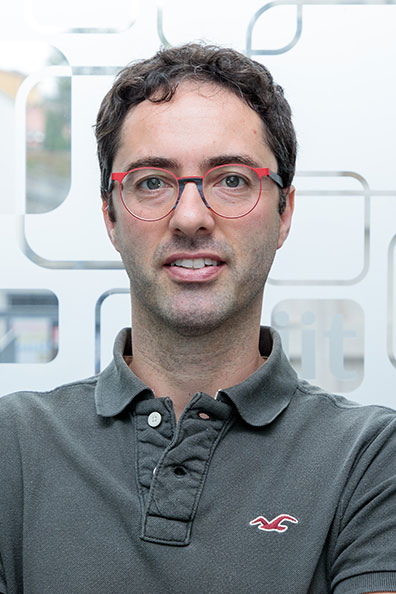
\includegraphics[scale=0.25]{papaleo}
	
\end{columns}



\end{frame}


\begin{frame}{Intracellular calcium dynamics}

\begin{columns}
	\column{0.45\linewidth}
	\begin{itemize}
		\vspace{0.5cm}
		\item Neurons show \textit{rapid} and \textit{heavy} changes in the values of their intracellular concentration of $Ca^{2+}$
		
		\vspace{0.5cm}
		
		\item The neuron is defined as \textit{active} in correspondence to the peaks in the calcium concentration
		
		
		
	\end{itemize}
	\column{0.45\linewidth}
	\centering
	\includegraphics[scale=0.4]{ca_conc}
	
\end{columns}

\end{frame}

\begin{frame}{Microendoscopic calcium imaging}



Te \textbf{Microendoscopic calcium imaging} technique consists in the following steps:

\begin{enumerate}
	
	\item Implant of \textit{miniscopes} in the brain region of interest of mice
	
	\item Injection of a virus carrying the \textbf{GCaMP} protein
	
	\item Performance of the behavioural task
	
	\item Collection of the video recordings of the fluorescence activity in single neurons
	
	\item Pre-processing and data analysis
\end{enumerate}

\begin{figure}[H]
	
	\centering
	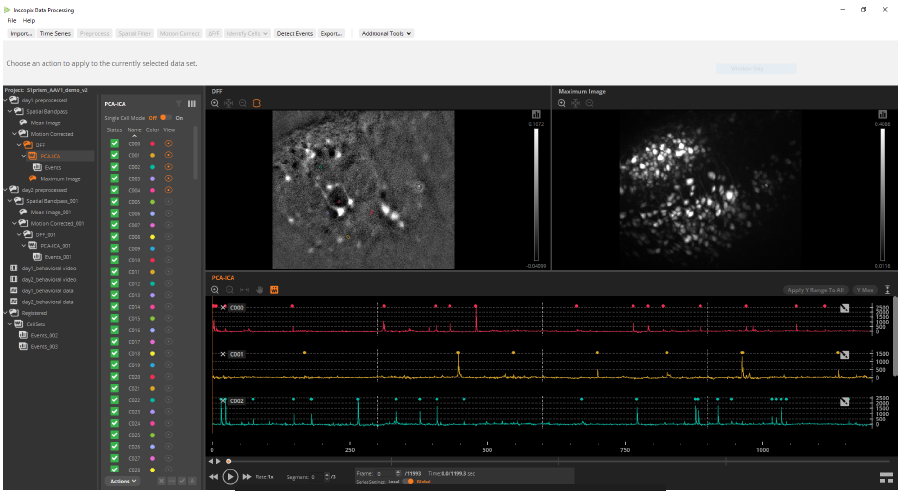
\includegraphics[width=0.25\textwidth]{inscopix}
	
\end{figure}
\end{frame}


\begin{frame}{Main projects}
\begin{itemize}
	\item Mathematical modeling of the calcium patterns occuring in a neuronal pair
	\vspace{0.5cm}
	\item \textbf{ Data analysis on the altruism task}: recording of $Ca^{2+}$ activity in the \textit{amygdala} during altruistic behaviours
	\vspace{0.5cm}
	\item \textbf{ Interbrain data analysis}: study of the synchronization between  neural activities of two mice

	
\end{itemize}
\end{frame}


\begin{frame}{Intebrain analysis for the EDT}
\textbf{Emotion discrimination task (EDT)}

\begin{columns}
	\column{0.5\linewidth}
	\begin{itemize}
		\vspace{0.5cm}
		\item An \textit{observer} mouse faces a \textit{neutral} and a \textit{stressed} demonstrator 
		
	
		\item Three phases of the task: \textit{homecage}, \textit{habituation}, \textit{test}
		
		
		\item Main goal: investigate synchronization between overall and single neuron activities between mice and correlations with emotional state
		
		
	\end{itemize}
	\column{0.75\linewidth}
	\centering
	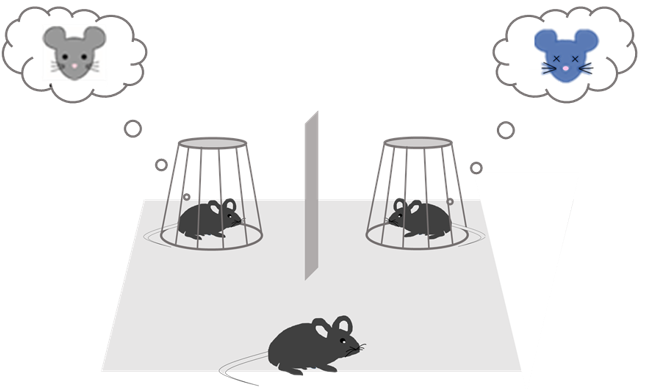
\includegraphics[scale=0.35]{emotion_discrimination}
	
\end{columns}

\end{frame}

\begin{frame}{Cross-Correlation analysis}
Considering the \textit{average activity} of the neurons, the synchronziation has been quantified using the \textbf{cross-correlation}.\\ Given two functions $ f = f(t)$ and $ g = g(t)$, we define the cross-correlation between them as

\vspace{1 cm}
$$
[f(t) \star g(t)] (\tau) = \int_{-\infty}^{+\infty} f(\tau)g(t+\tau) dt$$ \label{cc_def}


\end{frame}

\begin{frame}{Results on the cross-correlation analysis}

The cross-correlation peaks around $lag=0$ only for the interaction observer - neutral. Such result is not present in the control phases of homecage and habituation.


\begin{figure}[H]
	
	\centering
	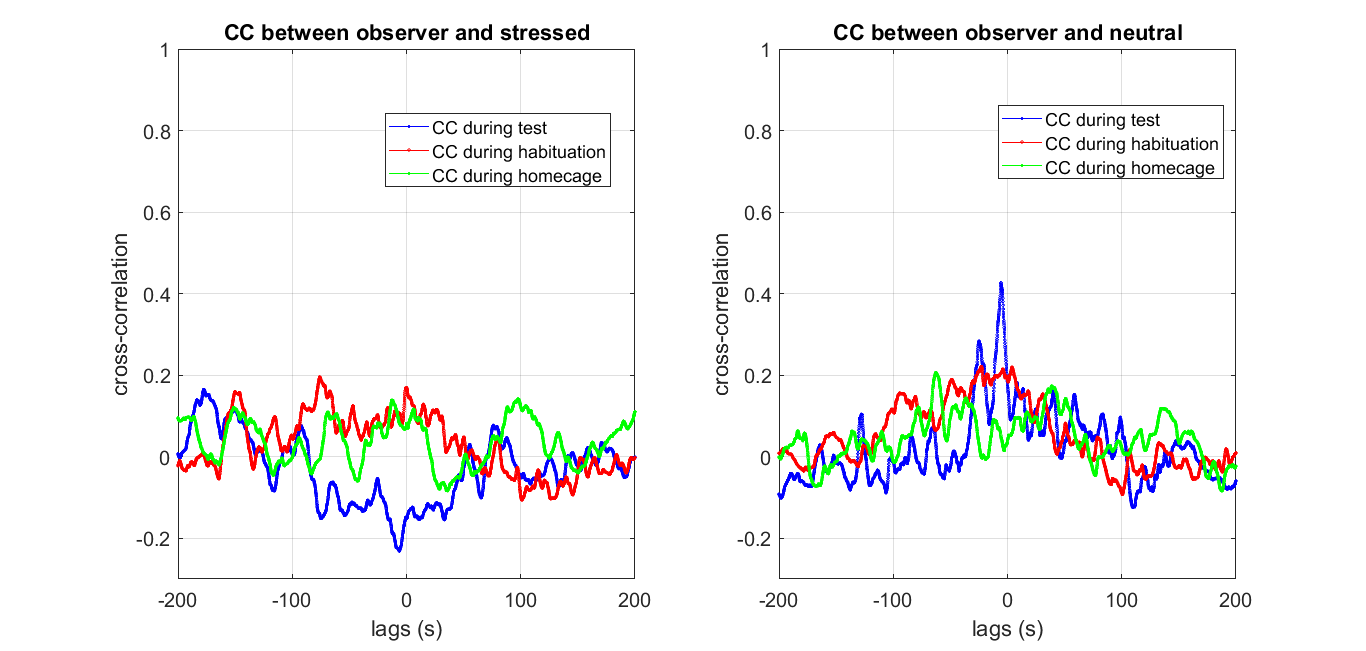
\includegraphics[scale=0.3]{average_cc}

\end{figure}
	
\end{frame}

\begin{frame}{Peak correlation analysis}
To quantify the amount of \textit{simultaneous peaks} occurred between the neurons of two different mice, we employ the \textbf{peak correlation index}

$$ i_{AB} = \frac{N_{AB} T}{2 N_A N_B dT} $$ 

Where: \begin{itemize}
	
	\item $T$ is the overall signals time window 
	
	\item $dT$ is the synchronization time window
	
	\item $N_A$ and $N_B$ are the number of peaks in signal A and B
	
	\item $N_{AB} = \sum_{i=1}^{N_A} \sum_{j=1}^{N_B} I_{[-dT,dT]}(|a_i - b_j|) $ is the sum of simulteneous peaks occurred between neurons A and B during the window $dT$
\end{itemize}


\end{frame}


\begin{frame}{Results on the peak correlation analysis}
In accordance with the cross-correlation result, the pair observer - neutral shows an increase in the average peak correlation index, computed across all neuronal pairs.

\begin{figure}[H]
	
	\centering
	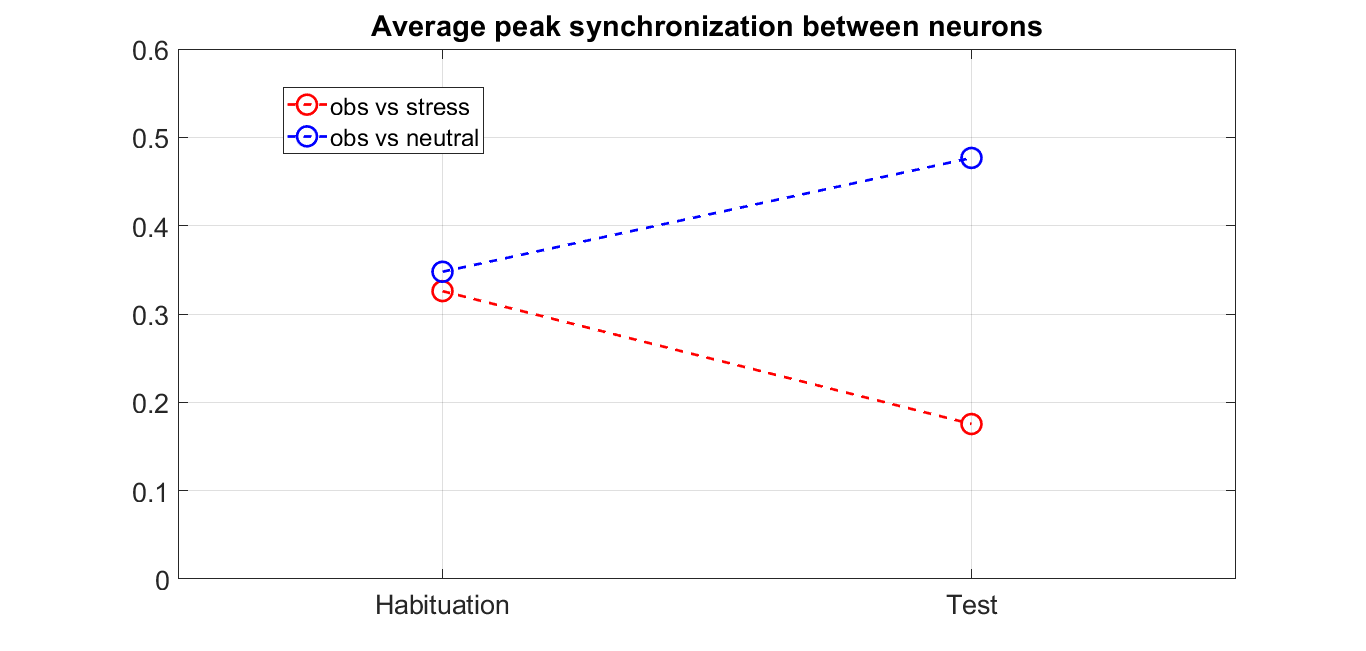
\includegraphics[scale=0.3]{avg_pks}
	
\end{figure}

\end{frame}


\begin{frame}{The self-experience task}
In the \textbf{self-experience} task, the observer is stressed before the beginning of the test. This provokes an \textit{inhibition} of the synchronization (cross- correlation and peak synchronization)

\begin{figure}[H]
	
	\centering
	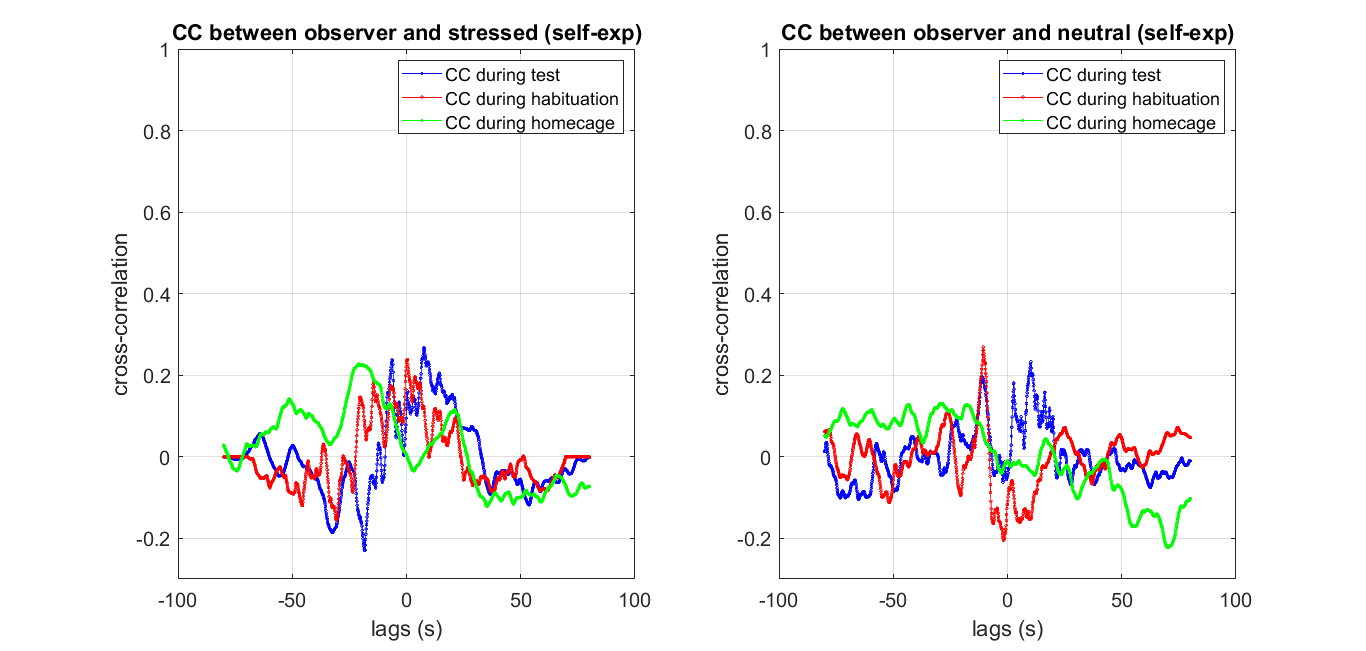
\includegraphics[scale=0.3]{average_cc_self}
	
\end{figure}
\end{frame}

\end{document}


\begin{frame}{The GECO group}

\movie[width=8cm,height=4.5cm]{test}{video2.mp4}

\end{frame}
	


\begin{figure}
	
	\hfill
	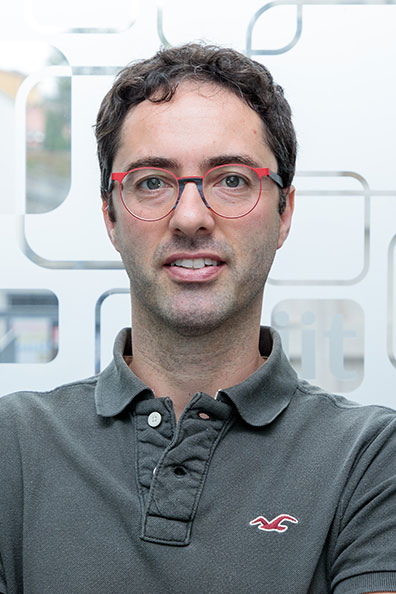
\includegraphics[width=0.25\textwidth]{papaleo.jpg}
	
\end{figure}


\begin{frame}{The GECO group}
	contenuto...
\end{frame}